\documentclass{article}
\usepackage{graphicx} % Required for inserting images

\usepackage[paper=a4paper,dvips,top=1.5cm,left=1.5cm,right=1.5cm,
    foot=1cm,bottom=1.5cm]{geometry}


\usepackage{todonotes}          %to provide inline and margin notes
%\usepackage[T1]{fontenc}
%%\usepackage{pslatex}
\renewcommand{\rmdefault}{ptm} 
\usepackage{mathptmx}
\usepackage[scaled=.90]{helvet}
\usepackage{courier}
%
\usepackage{bookmark}

\usepackage{fancyhdr}
\pagestyle{fancy}

%%----------------------------------------------------------------------------
%%   pcap2tex stuff
%%----------------------------------------------------------------------------
 %%\usepackage[dvipsnames*,svgnames]{xcolor} %% For extended colors
 %%\usepackage{tikz}  %% Already loaded
 %%\usetikzlibrary{arrows,decorations.pathmorphing,backgrounds,fit,positioning,calc,shapes}

%% \usepackage{pgfmath}	% --math engine
%%----------------------------------------------------------------------------
%% \usepackage[latin1]{inputenc}
\usepackage[utf8]{inputenc} % inputenc allows the user to input accented characters directly from the keyboard
\usepackage[english]{babel}
%% \usepackage{rotating}		 %% For text rotating
\usepackage{array}			 %% For table wrapping
\usepackage{graphicx}	                 %% Support for images
\usepackage{float}			 %% Suppor for more flexible floating box positioning
\usepackage{color}                       %% Support for colour 
\usepackage{mdwlist}
%% \usepackage{setspace}                 %% For fine-grained control over line spacing
%% \usepackage{listings}		 %% For source code listing
%% \usepackage{bytefield}                %% For packet drawings
\usepackage{tabularx}		         %% For simple table stretching
%%\usepackage{multirow}	                 %% Support for multirow colums in tables
\usepackage{dcolumn}	                 %% Support for decimal point alignment in tables
\usepackage{url}	                 %% Support for breaking URLs
\usepackage[perpage,para,symbol]{footmisc} %% use symbols to ``number'' footnotes and reset which symbol is used first on each page
\usepackage{siunitx} %% to be able to use binary units
\newcommand{\SIadj}[2]{\SI[number-unit-product={\text{-}}]{#1}{#2}}

%% \usepackage{pygmentize}           %% required to use minted -- see python-pygments - Pygments is a Syntax Highlighting Package written in Python
%% \usepackage{minted}		     %% For source code highlighting

%% \usepackage{hyperref}		
\usepackage[all]{hypcap}	 %% Prevents an issue related to hyperref and caption linking
%% setup hyperref to use the darkblue color on links
%% \hypersetup{colorlinks,breaklinks,
%%             linkcolor=darkblue,urlcolor=darkblue,
%%             anchorcolor=darkblue,citecolor=darkblue}

%% Some definitions of used colors
\definecolor{darkblue}{rgb}{0.0,0.0,0.3} %% define a color called darkblue
\definecolor{darkred}{rgb}{0.4,0.0,0.0}
\definecolor{red}{rgb}{0.7,0.0,0.0}
\definecolor{lightgrey}{rgb}{0.8,0.8,0.8} 
\definecolor{grey}{rgb}{0.6,0.6,0.6}
\definecolor{darkgrey}{rgb}{0.4,0.4,0.4}
%% Reduce hyphenation as much as possible
\hyphenpenalty=15000 
\tolerance=1000

%% useful redefinitions to use with tables
\newcommand{\rr}{\raggedright} %% raggedright command redefinition
\newcommand{\rl}{\raggedleft} %% raggedleft command redefinition
\newcommand{\tn}{\tabularnewline} %% tabularnewline command redefinition

%% definition of new command for bytefield package
\newcommand{\colorbitbox}[3]{%
	\rlap{\bitbox{#2}{\color{#1}\rule{\width}{\height}}}%
	\bitbox{#2}{#3}}

%% command to ease switching to red color text
\newcommand{\red}{\color{red}}
%%redefinition of paragraph command to insert a breakline after it
\makeatletter
\renewcommand\paragraph{\@startsection{paragraph}{4}{\z@}%
  {-3.25ex\@plus -1ex \@minus -.2ex}%
  {1.5ex \@plus .2ex}%
  {\normalfont\normalsize\bfseries}}
\makeatother

%%redefinition of subparagraph command to insert a breakline after it
\makeatletter
\renewcommand\subparagraph{\@startsection{subparagraph}{5}{\z@}%
  {-3.25ex\@plus -1ex \@minus -.2ex}%
  {1.5ex \@plus .2ex}%
  {\normalfont\normalsize\bfseries}}
\makeatother

\setcounter{tocdepth}{3}	%% 3 depth levels in TOC
\setcounter{secnumdepth}{5}
%% Acronyms
\usepackage[acronym, nopostdot]{glossaries}
\glsdisablehyper
%\makeglossaries

\renewcommand{\headrulewidth}{0pt}
%%%%%%%%%%%%%%%%%%%%%%%%%%%%%%%%%%%%%%%%%%%%%%%%%%%%%%%%%%%%%%%%%%%%
%% End of preamble
%%%%%%%%%%%%%%%%%%%%%%%%%%%%%%%%%%%%%%%%%%%%%%%%%%%%%%%%%%%%%%%%%%%%
\usepackage{verbatim}
\newcommand{\detailtexcount}[1]{%
  \immediate\write18{texcount -merge -sum -q #1.tex output.bbl > #1.wcdetail }%
  \verbatiminput{#1.wcdetail}%
}
\newcommand{\quickwordcount}[1]{%
  \immediate\write18{texcount -1 -sum -merge -q #1.tex output.bbl > #1-words.sum }%
  \input{#1-words.sum} words%
}

\usepackage{multicol}
\usepackage{wasysym}

\usepackage[english]{isodate}

\newacronym{ACK}{ACK}{Acknowledgement}
\newacronym{KTH}{KTH}{KTH Royal Institute of Technology}
\newacronym{NACK}{NACK}{Negative Acknowledgement}
\newacronym{UDP}{UDP}{User Datagram Protocol}



\title{Labbrapport}
\author{viktor björkén }
\date{Maj 2023}

\begin{document}

\maketitle

\section{Kortet}

Jag har valt att göra en s.k. "Step-Down Converter" baserat på TPS5430 chippet.
Jag har under konstruktionens gång följt en \textit{Evaluation Module User's
Guide} ifrån Texas Instruments. Det som skiller kretsen från det tidigare
nämnda databladet är att jag har valt att addera funktionen som gör det möjligt
att välja vilket volt värde man vill få ut. 

\begin{figure}[htp]
    \centering
    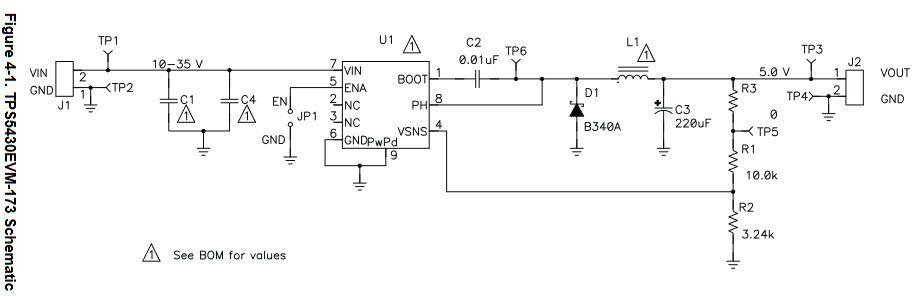
\includegraphics[width=15cm]{img/nyschema.png}
    \caption{Bild av schematic från slvu157a datablad}
\end{figure}

För att kretsen ska kunna välja bland flera output volt värden, behöver vi
kunna ändra värdet på R2 resistorn som tillsammans med R1 bygger upp en
spänningsdelare.

\begin{figure}[htp]
    \centering
    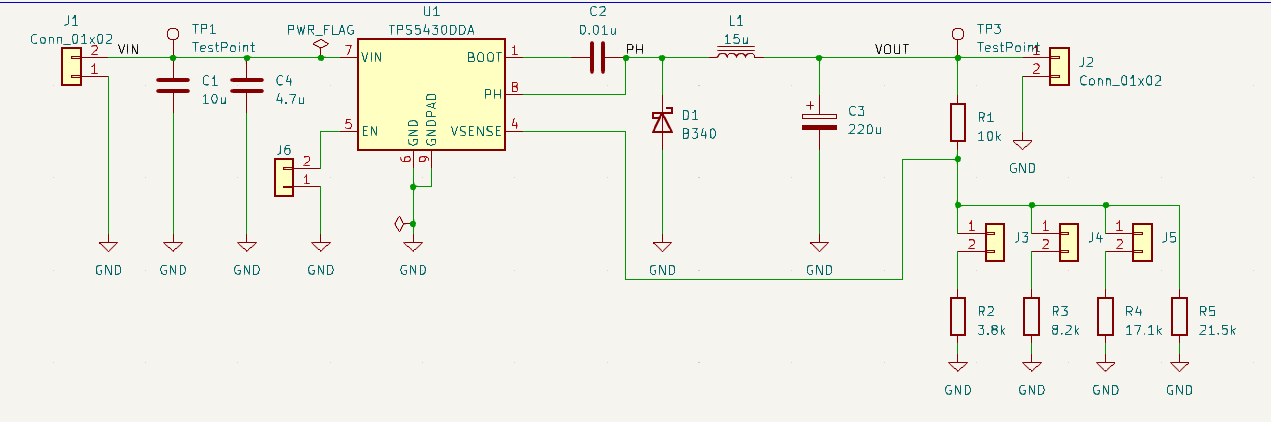
\includegraphics[width=15cm]{img/schemalab.png}
    \caption{Bild av schematic från kiCad}
\end{figure}


\section{PCB layout}

När jag designade kretsen valde jag att så noga som möjligt följa databladet och dess
rekomendationer. I miitt första utkast hade jag vanliga "sladdar" mellan alla komponenter
men sedan efter feedback valde jag att göra kortet på samma sätt som i databladet med 
koppar plattor mellan de olika ytorna. Jag la också till EN benet från IC, där man
beroende på om den kopplas till jord eller är flytande ger olika funktionalitet. 

\begin{figure}[htp]
    \centering
    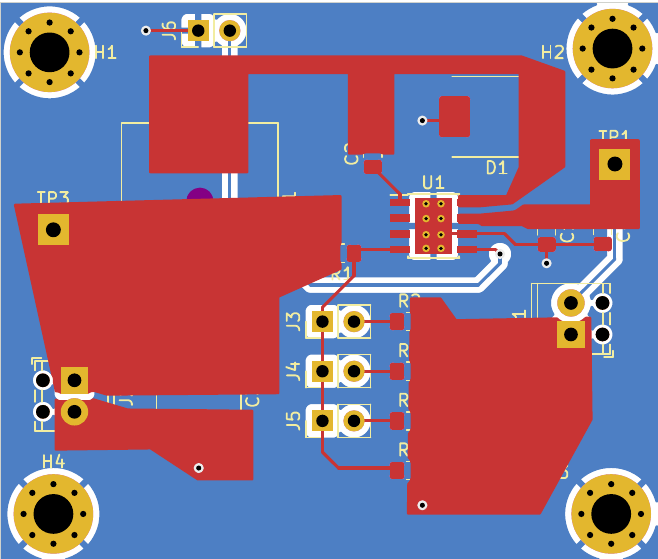
\includegraphics[width=10cm]{img/nylayout.png}
    \caption{Bild av schematic från kiCad}
\end{figure}

\begin{figure}[htp]
    \centering
    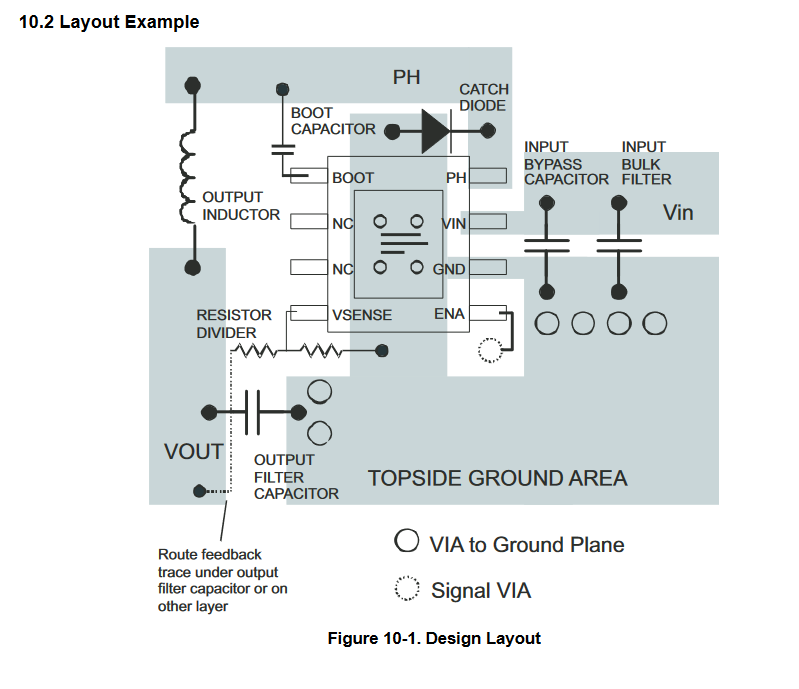
\includegraphics[width=10cm]{img/layout.png}
    \caption{Bild av layout från datablad}
\end{figure}

\section{BOM}

Här under finns min BOM lista med de olika komponenter jag använt mig utav, alla delar gick
inte att få tag i vilket gjorde att jag inte kunde färdligställa kortet.

\begin{figure}[htp]
\centering
\includegraphics[width=10cm]{img/bom.png}
\caption{BOM lista}
\end{figure}

\section{Slutprodukt}
Jag hann inte att löda på flera komponeter på mitt kort vilket såklart är väldigt tråkigt
jag var inte så stadig på handen vilket gjorde att det tog en del tid med ytmonterade 
komponenter. Som tidigare nämnt hade jag dessutom inte alla kompontenter vilket resulterade
i att jag inte kände behover att fortsätta löda vid ett senare tillfälle då den ändå 
inte skulle slutföras.

\begin{figure}[htp]
\centering
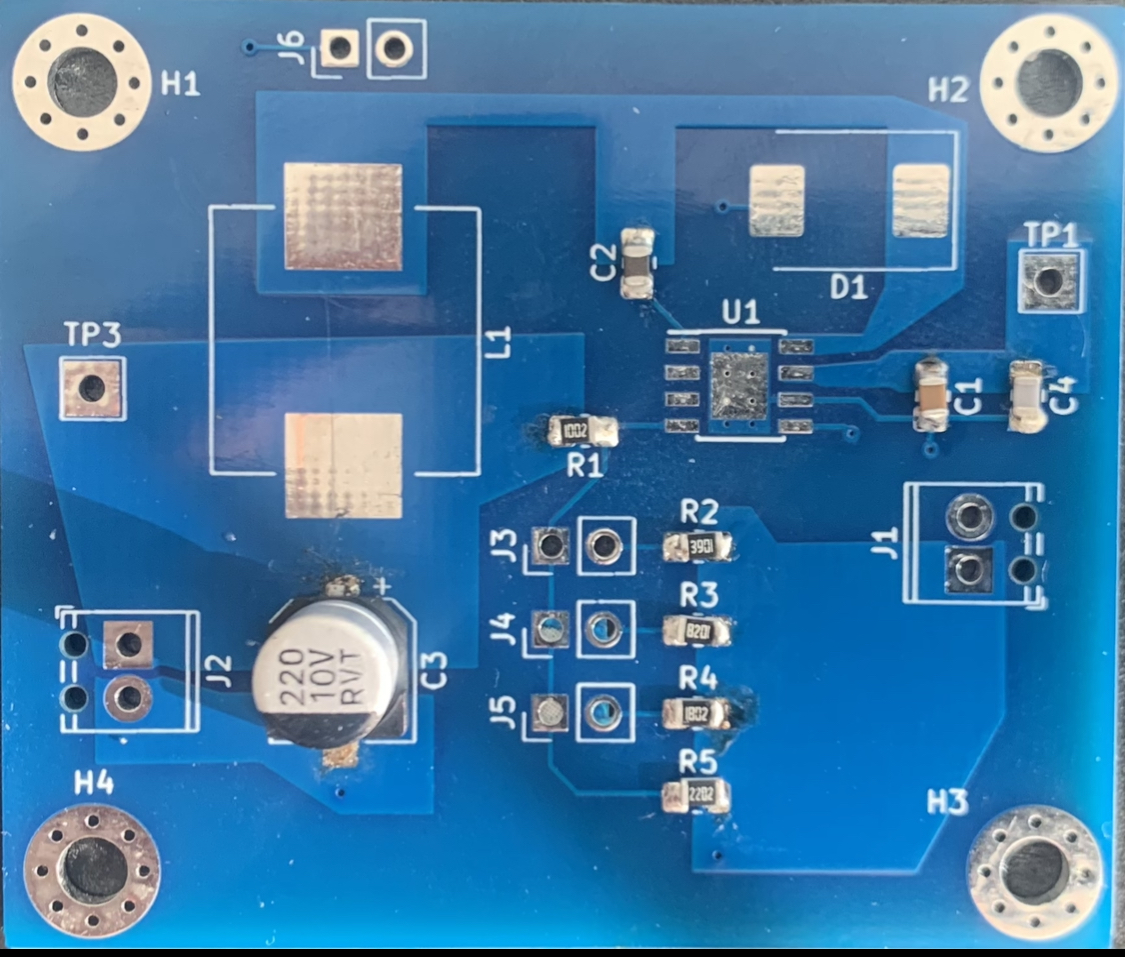
\includegraphics[width=10cm]{img/irlkort.jpeg}
\caption{BOM lista}
\end{figure}

\end{document}

